\section{PROCEDIMIENTO} 

\begin{itemize}
\subsection{Parte 1: Iniciando Docker}
	\item Abrir el menu inicio y buscar la aplicación Docker for Windows.

	\item Ubicar la aplicación PowerShell, ejecutarla como Administrador. En la ventana de comandos de PowerShell escribir
lo siguiente.
		\begin{figure}[H]
		\begin{center}
		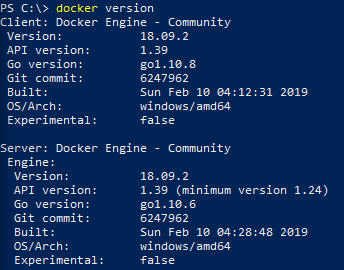
\includegraphics[width=8cm]{./Imagenes/1}
		\end{center}
		\end{figure}
     
\subsection{Parte 2: Creando un contenedor con Oracle Database para Linux}
	\item En un navegador de internet acceder a la dirección https://hub.docker.com/. Iniciar sesión o crear una cuenta nueva
	\item Buscar el repositorio para Oracle Database. Ingresar y proceder con el CheckOut, completar los datos y aceptar las condiciones obligatorias para obtener el acceso al contenido.
		\begin{figure}[H]
		\begin{center}
		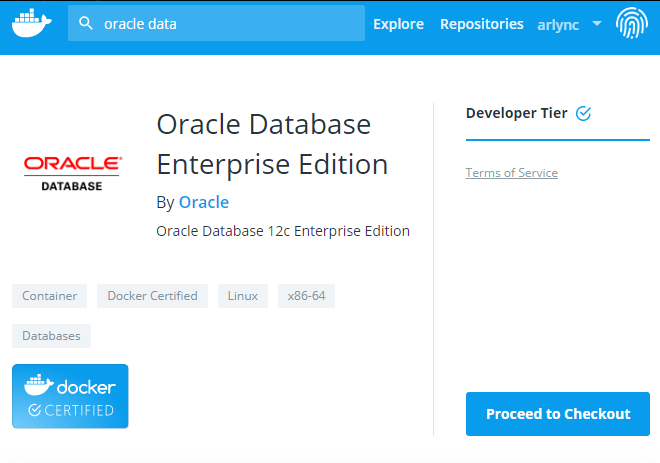
\includegraphics[width=8cm]{./Imagenes/3}
		\end{center}
		\end{figure}
	\item En la ventana de PowerShell, escribir el siguiente comando:
		\begin{figure}[H]
		\begin{center}
		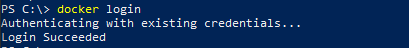
\includegraphics[width=9cm]{./Imagenes/4}
		\end{center}
		\end{figure}
	\item Ejecutar el siguiente comando en Powershell, lo cual descargará la imagen del contenedor de Oracle Database en un servidor Linux
		\begin{figure}[H]
		\begin{center}
		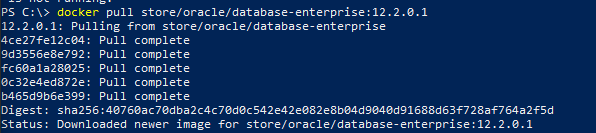
\includegraphics[width=15cm]{./Imagenes/5}
		\end{center}
		\end{figure}
	\item Seguidamente ejecutar el comando, como respuesta se visualizará un ID que corresponde al contenedor.
		\begin{figure}[H]
		\begin{center}
		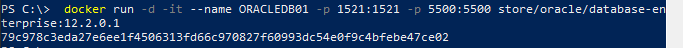
\includegraphics[width=15cm]{./Imagenes/6}
		\end{center}
		\end{figure}
	\item Verificar que el contenedor se esté ejecutando correctamente mediante el comando:
		\begin{figure}[H]
		\begin{center}
		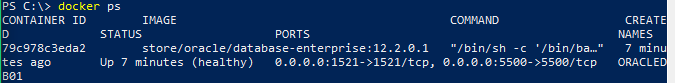
\includegraphics[width=15cm]{./Imagenes/7}
		\end{center}
		\end{figure}
	\item Cuando el estado del contenedor sea “healthy”, en la consola de Powershell, ejecutar el siguiente comando:
		\begin{figure}[H]
		\begin{center}
		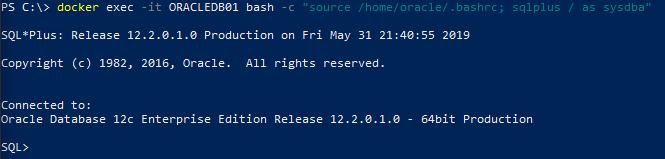
\includegraphics[width=15cm]{./Imagenes/8}
		\end{center}
		\end{figure}
	\item En la línea de comentados de SQL*Plus, escribir lo siguiente
		\begin{figure}[H]
		\begin{center}
		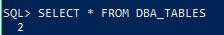
\includegraphics[width=8cm]{./Imagenes/9}
		\end{center}
		\end{figure}
	\item Escribir el comando quit para cerrar la sesión de SQL*Plus
		\begin{figure}[H]
		\begin{center}
		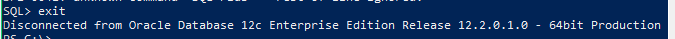
\includegraphics[width=15cm]{./Imagenes/10}
		\end{center}
		\end{figure}
	\item En una pestaña nueva del navegador de internet acceder a la siguiente dirección:https://localhost:5500/em. Iniciar sesión con los siguientes datos:
		\begin{figure}[H]
		\begin{center}
		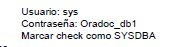
\includegraphics[width=4cm]{./Imagenes/t1}
		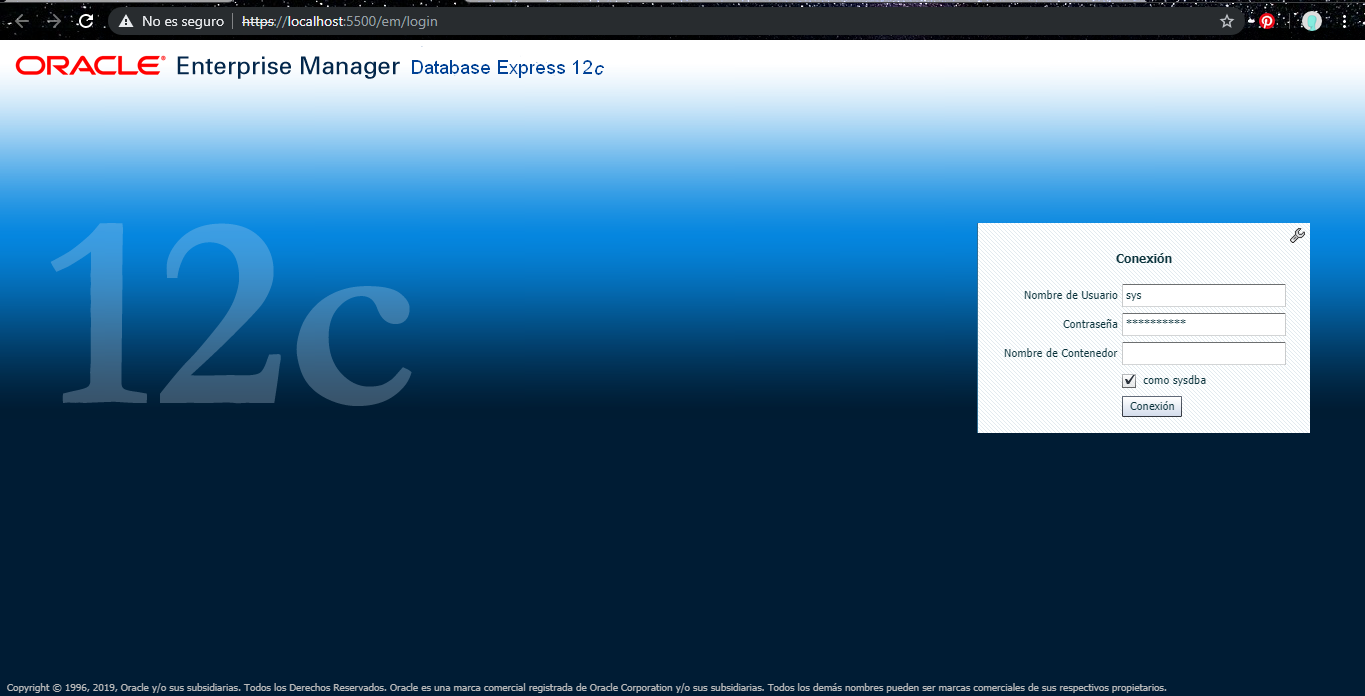
\includegraphics[width=15cm]{./Imagenes/11}
		\end{center}
		\end{figure}
	\item Luego se visualizará la siguiente ventana. Cerrar sesión y la pestaña del navegador de internet.
		\begin{figure}[H]
		\begin{center}
		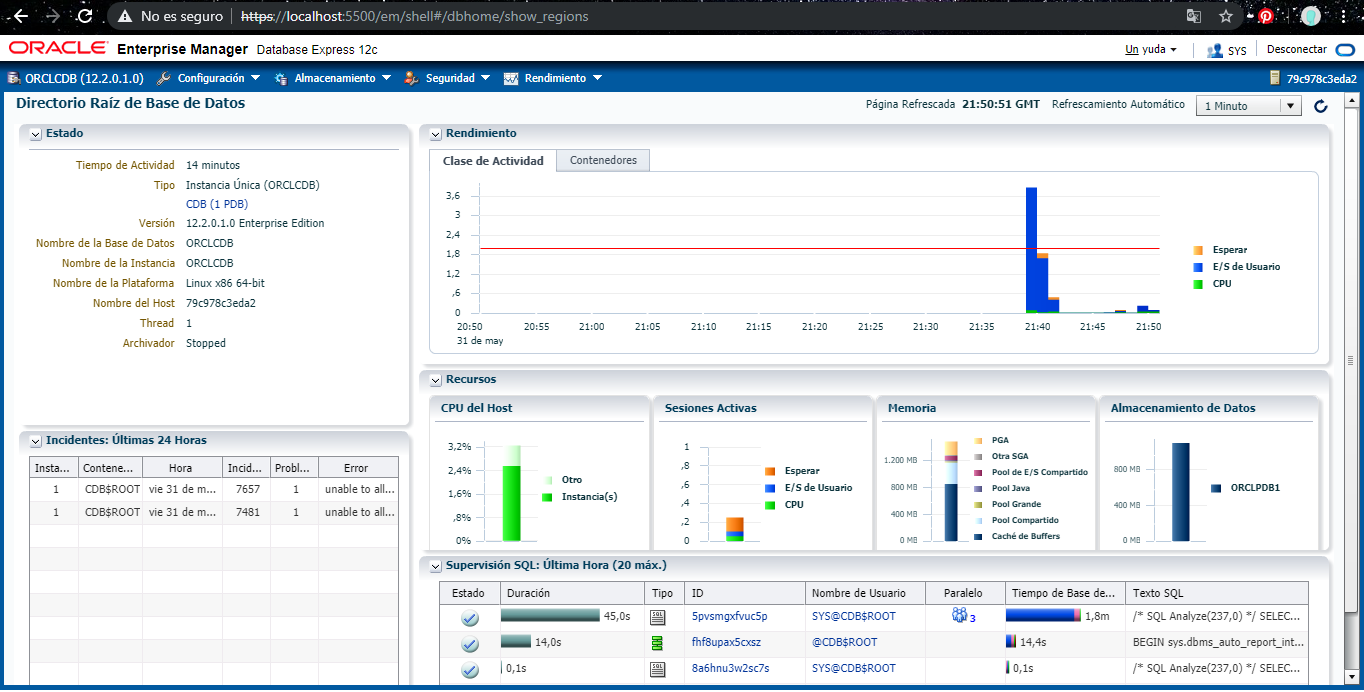
\includegraphics[width=15cm]{./Imagenes/12}
		\end{center}
		\end{figure}
	\item Iniciar el aplicativo Oracle SQL Developer, crear una nueva conexión con los siguientes parámetros:
		\begin{figure}[H]
		\begin{center}
		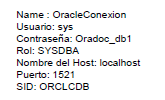
\includegraphics[width=5cm]{./Imagenes/t2}
		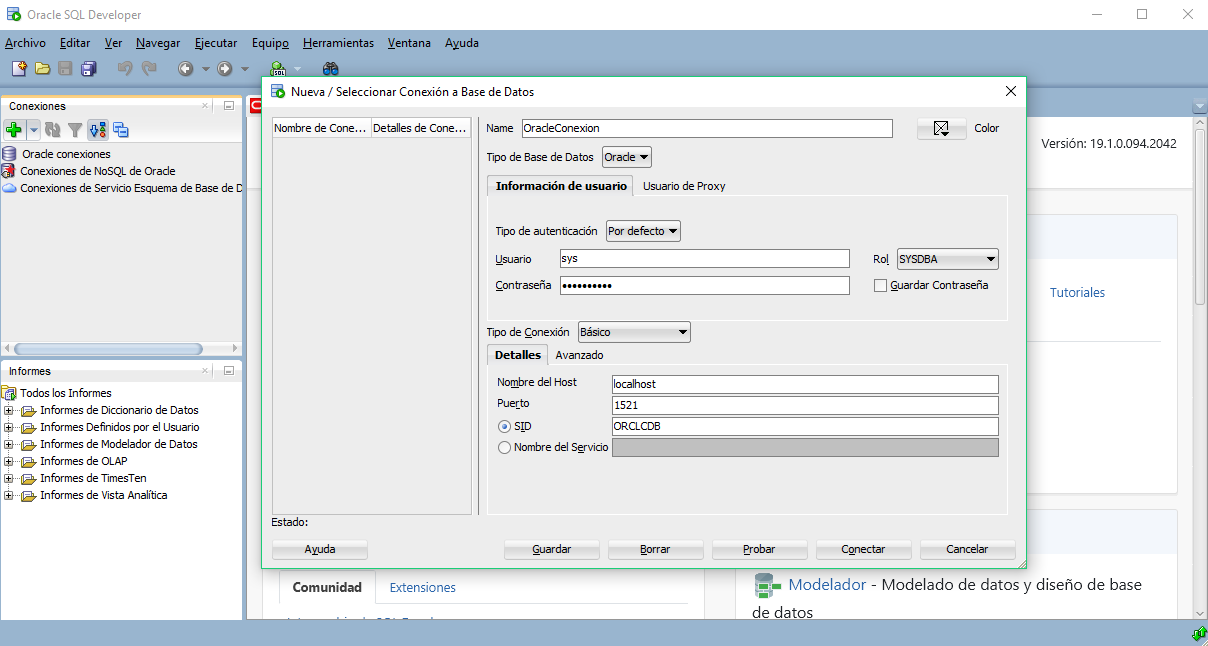
\includegraphics[width=15cm]{./Imagenes/13}
		\end{center}
		\end{figure}
	\item Iniciar una nueva consulta, escribir y ejecutar lo siguiente; deberá retornar varios registros que representan las tablas de las base de datos
		\begin{figure}[H]
		\begin{center}
		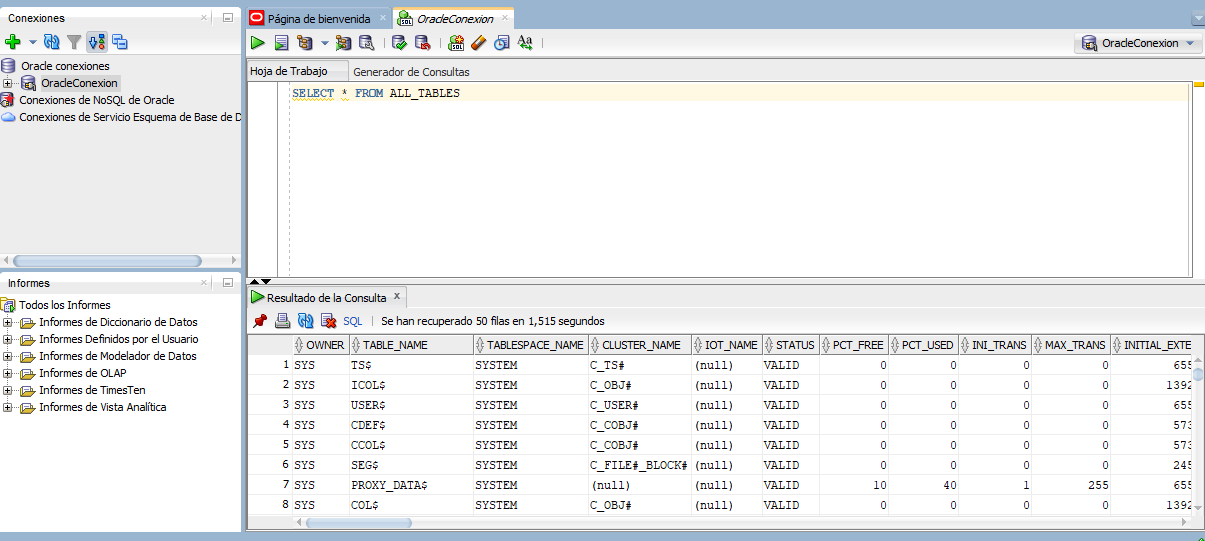
\includegraphics[width=15cm]{./Imagenes/14}
		\end{center}
		\end{figure}
	\item Cerrar la aplicación Oracle SQL Developer
	\item En PowerShell ejecutar el siguiente comando. Y verificar la eliminación del contenedor con ejecutando
		\begin{figure}[H]
		\begin{center}
		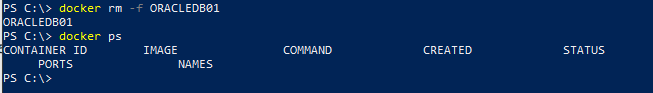
\includegraphics[width=12cm]{./Imagenes/15}
		\end{center}
		\end{figure}


\subsection{Parte 3: Adicionando persistencia}
	\item Abrir el menu inicio y buscar la aplicación Docker for Windows.
       
\end{itemize}
		